\subsection{\texorpdfstring{同态 \(\operatorname{Tor}_n^{\mathbf{A}}(\mathbf{P},\mathbf{M})\to \operatorname{Hom}_{\mathbf{A}}(\operatorname{Ext}_{\mathbf{A}}^{n}(\mathbf{M},\mathbf{A}),\mathbf{P})\)}{同态 \textbackslash operatorname\{Tor\}\_n\^{}\{\textbackslash mathbf\{A\}\}(\textbackslash mathbf\{P\},\textbackslash mathbf\{M\})\textbackslash 到 \textbackslash operatorname\{Hom\}\_\{\textbackslash mathbf\{A\}\}(\textbackslash operatorname\{Ext\}\_\{\textbackslash mathbf\{A\}\}\^{}\{n\}(\textbackslash mathbf\{M\},\textbackslash mathbf\{A\}),\textbackslash mathbf\{P\})}}

设 M 为左 A-模，P 为右 A-模，且 n 为整数 \(\geqslant 0\) 。k-双线性映射（X，第 129 页）

\[
c _ {\mathrm{P}; \mathrm{M}, \mathrm{A} _ {s}}: \operatorname{Ext} _ {\mathrm{A}} ^ {n} (\mathrm{M}, \mathrm{A}) \times \operatorname{Tor} _ {n} ^ {\mathrm{A}} (\mathrm{P}, \mathrm{M}) \rightarrow \mathrm{P} \otimes_ {\mathrm{A}} \mathrm{A}
\]

对应于一个 k-线性映射

\[
\operatorname{Tor} _ {n} ^ {\mathbf {A}} (\mathrm{P}, \mathrm{M}) \rightarrow \operatorname{Hom} _ {k} \left(\operatorname{Ext} _ {\mathbf {A}} ^ {n} (\mathrm{M}, \mathrm{A}), \mathrm{P}\right);\tag{2}
\]

此外，若给 Ext \(_{A}^{n}\) （M，A）赋以由 A 的双模结构产生的右 A-模结构，则（2）的像由 A-线性映射组成，这一点可立即验证；由此可推出一个 k-同态，称为典范的

\[
\operatorname{Tor} _ {n} ^ {\mathbf {A}} (\mathrm{P}, \mathrm{M}) \rightarrow \operatorname{Hom} _ {\mathbf {A}} \left(\operatorname{Ext} _ {\mathbf {A}} ^ {n} (\mathrm{M}, \mathrm{A}), \mathrm{P}\right).\tag{3}
\]

命题 3. --- a) 若 \(\mathrm{dp}_{\mathbf{A}}(\mathbf{M}) \leqslant n\) ，则典范同态 (3) 是单射。 b) 若 \(\mathrm{dp}_{\mathbf{A}}(\mathbf{M}) \leqslant n\) ，且 A 是左诺特环、M 是有限生成的，则典范同态 (3) 是双射。

让我们对 \(n\) 进行归纳。如果 \(n = 0\) ，M 是投射的，同态 (3) 归结为典范同态 \(\mathbf{P} \otimes_{\mathbf{A}} \mathbf{M} \to \operatorname{Hom}_{\mathbf{A}} (\mathbf{M}^{*}, \mathbf{P})\) （见 II，第 77 页），命题由该处的推论得出。若 \(n > 0\) ，设

\[
0 \rightarrow \mathbf {N} \rightarrow \mathbf {L} \rightarrow \mathbf {M} \rightarrow 0\tag{4}
\]

是 A-模的正合序列，其中 L 是自由的（在情形 b) 中有限生成）；则 \(\mathrm{dp}_{\mathbf{A}}(\mathbf{N}) \leqslant n - 1\) （X，第 135 页，推论 2, c)），且在情形 b) 中 N 是有限生成的。

设 \(\theta\in\mathrm{Ext}_{\mathbf{A}}^{1}(\mathbf{M},\mathbf{N})\) 为与正合序列 (4) 相关联的类（X，第 117 页，定义 1）。用

\[
u _ {n}: \operatorname{Ext} _ {\mathbf {A}} ^ {n - 1} (\mathrm{N}, \mathrm{A}) \rightarrow \operatorname{Ext} _ {\mathbf {A}} ^ {n} (\mathrm{M}, \mathrm{A}) \quad v _ {n}: \operatorname{Tor} _ {n} ^ {\mathbf {A}} (\mathrm{P}, \mathrm{M}) \rightarrow \operatorname{Tor} _ {n - 1} ^ {\mathbf {A}} (\mathrm{P}, \mathrm{N})
\]

\[
(\alpha \circ \theta) \circ \beta = \alpha \circ (\theta \circ \beta)
\]

表示由 \(u_{n}(\alpha) = \alpha \circ \theta\) 与 \(v_{n}(\beta) = \theta \circ \beta\) 定义的映射。对所有 \(\alpha\in\mathrm{Ext}_{\mathbf{A}}^{n-1}\left(\mathbf{N},\mathbf{A}\right)\) , \(\beta\in\mathrm{Tor}_{n}^{\mathbf{A}}\left(\mathbf{P},\mathbf{M}\right)\left(\mathbf{X},\text{p. 129, prop. 6}\right)\) ，使得图表

\[
\begin{array}{c c c} \operatorname{Tor} _ {n} ^ {\mathbf {A}} (\mathrm{P}, \mathrm{M}) & \longrightarrow & \operatorname{Hom} _ {\mathbf {A}} \left(\operatorname{Ext} _ {\mathbf {A}} ^ {n} (\mathrm{M}, \mathrm{A}), \mathrm{P}\right) \\ \Big \downarrow v _ {n} & & \operatorname{Hom} (u _ {n}, 1) \Big \downarrow \\ \operatorname{Tor} _ {n - 1} ^ {\mathbf {A}} (\mathrm{P}, \mathrm{N}) & \longrightarrow & \operatorname{Hom} _ {\mathbf {A}} \left(\operatorname{Ext} _ {\mathbf {A}} ^ {n - 1} (\mathrm{N}, \mathrm{A}), \mathrm{P}\right), \end{array}\tag{5}
\]

其中水平箭头是典范同态，是交换的。若 n = 1，则我们有一个交换图表：

\pandocbounded{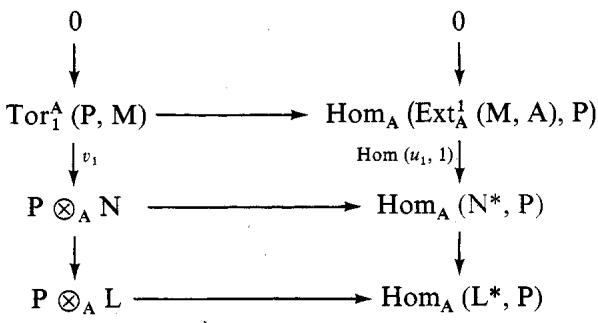
\includegraphics[keepaspectratio]{images/part001_66a54857.jpg}}

其中各列是正合的；在这种情况下我们推出结论。若 \(n \geqslant 2\) ，映射 \(u_n\) 与 \(v_n\) 是双射的（X，第 128 页，推论 4 及第 131 页，推论 3）。由归纳假设，典范同态

\[
\operatorname{Tor} _ {n - 1} ^ {\mathbf {A}} (\mathrm{P}, \mathrm{N}) \rightarrow \operatorname{Hom} _ {\mathbf {A}} \left(\operatorname{Ext} _ {\mathbf {A}} ^ {n - 1} (\mathrm{N}, \mathrm{A}), \mathrm{P}\right)
\]

是单射（相应地，双射）；图表（5）表明典范同态 \(\mathrm{Tor}_{n}^{\mathrm{A}}(\mathrm{P},\mathrm{M})\to \mathrm{Hom}_{\mathrm{A}}(\mathrm{Ext}_{\mathrm{A}}^{n}(\mathrm{M},\mathrm{A}),\mathrm{P})\) 也具有同样的性质，这完成了证明。

